% =====================================================================
%  Full-page nested-bracket hierarchy of a UI tree.
%
%  Containment encodes parent/descendant: a left bracket [ encloses a
%  node together with its whole subtree.  Each node sits at the TOP of
%  its own bracket; the bracket's bottom extends a fixed margin BELOW
%  its last child's bracket, so children nest neatly within the parent.
%  Depth = horizontal indent; preorder = vertical order.
%
%  Requires only \usepackage{tikz} and amssymb (\mathbb, \vartriangleleft).
% =====================================================================
% vertical bar + bottom serif of an elongated "["  (top = serif-to-label line)
\providecommand{\lbr}[4]{\draw[#1] (#2,#3) -- (#2,#4) -- ([xshift=4mm]#2,#4);}

\clearpage
\thispagestyle{empty}
\null\vfill
\noindent
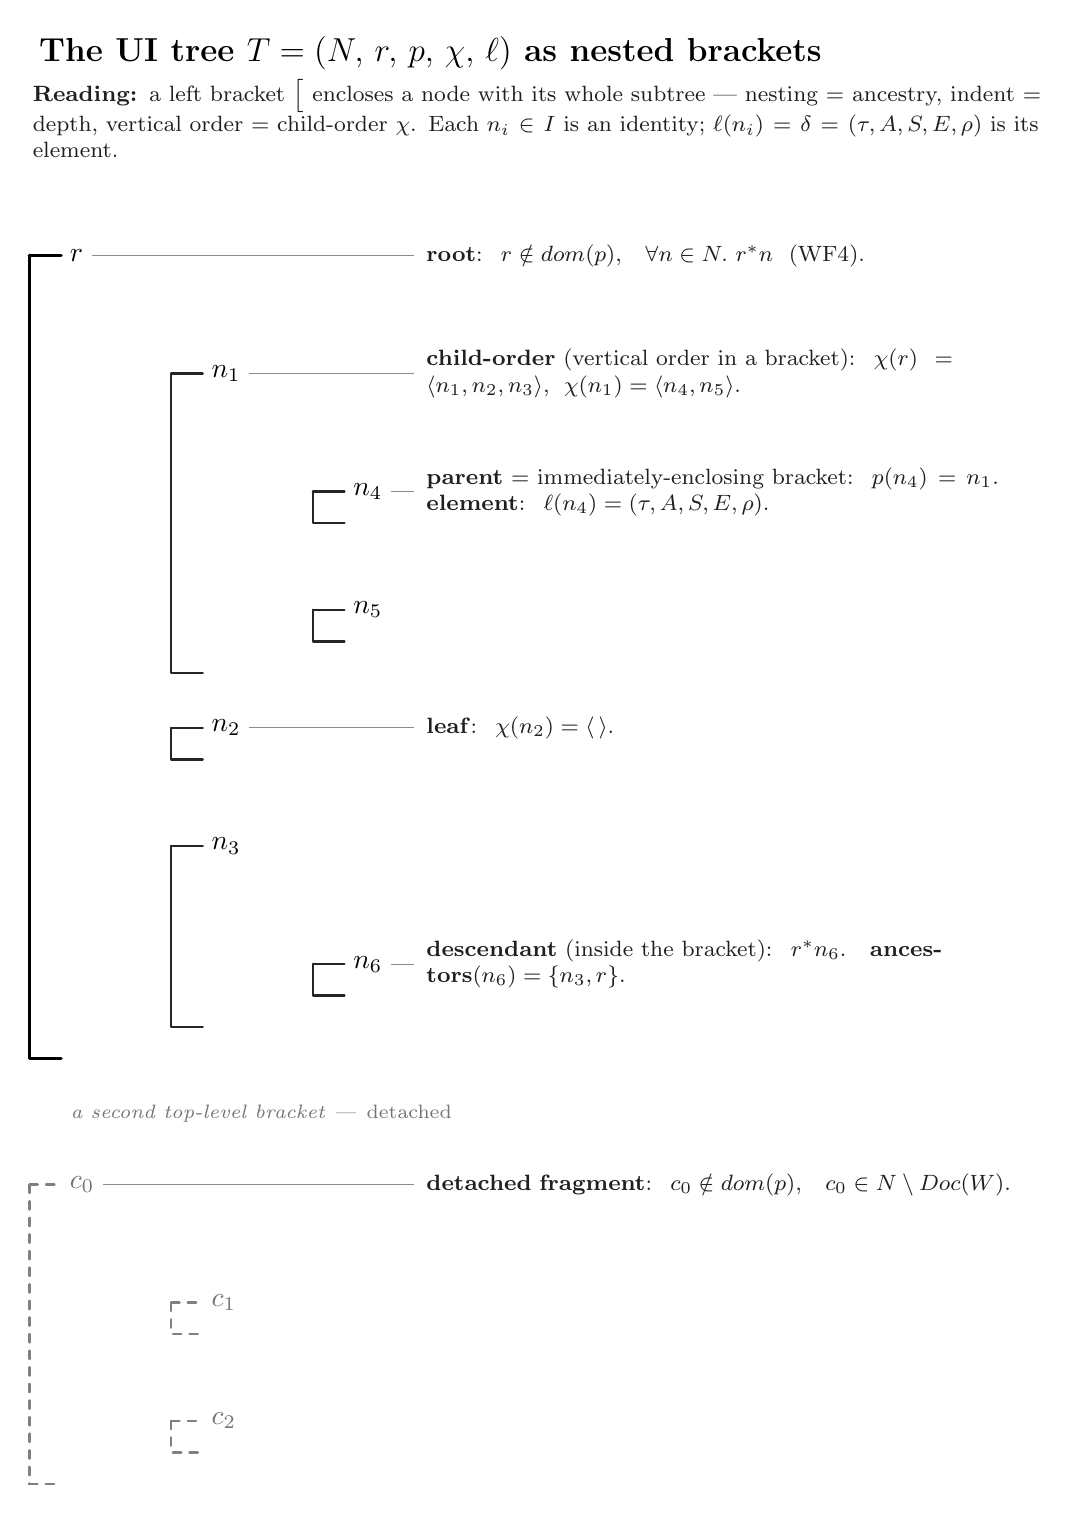
\begin{tikzpicture}[
  font=\footnotesize,
  nd/.style={anchor=west, inner xsep=3pt, inner ysep=1pt, font=\normalsize},
  ndd/.style={anchor=west, inner xsep=3pt, inner ysep=1pt, font=\normalsize, text=black!55},
  ann/.style={anchor=west, text width=7.6cm, align=left, font=\footnotesize,
              text=black!88, inner sep=1pt},
  leader/.style={draw=black!45, line width=.4pt},
  bk/.style={draw=black!85, line width=.9pt, line cap=round, line join=round},
  bkroot/.style={draw=black, line width=1.3pt, line cap=round, line join=round},
  bkd/.style={draw=black!50, line width=.9pt, dashed, line cap=round},
]

% ---------------- title + short reading guide ----------------
\node[font=\large\bfseries, anchor=north west] at (0,2.9)
  {The UI tree $T=(N,\,r,\,p,\,\chi,\,\ell)$ as nested brackets};
\node[ann, anchor=north west, text width=13.0cm] at (0,2.3)
  {\textbf{Reading:} a left bracket $\big[$ encloses a node with its whole subtree —
   nesting $=$ ancestry, indent $=$ depth, vertical order $=$ child-order $\chi$.
   Each $n_i\in\mathbb{I}$ is an identity; $\ell(n_i)=\delta=(\tau,A,S,E,\rho)$ is its element.};

% ---------------- node labels (sit on the top serif of each bracket) ----------------
\node[nd]  (r)  at (0.4,  0.0) {$r$};
\node[nd]  (n1) at (2.2, -1.5) {$n_1$};
\node[nd]  (n4) at (4.0, -3.0) {$n_4$};
\node[nd]  (n5) at (4.0, -4.5) {$n_5$};
\node[nd]  (n2) at (2.2, -6.0) {$n_2$};
\node[nd]  (n3) at (2.2, -7.5) {$n_3$};
\node[nd]  (n6) at (4.0, -9.0) {$n_6$};
\node[ndd] (c0) at (0.4,-11.8) {$c_0$};
\node[ndd] (c1) at (2.2,-13.3) {$c_1$};
\node[ndd] (c2) at (2.2,-14.8) {$c_2$};
\node[anchor=west, font=\scriptsize\itshape, text=black!55] at (0.4,-10.9)
  {a second top-level bracket — \emph{detached}};

% ---------------- brackets (bottom extends 0.4 below the last child's bottom) ----------------
\lbr{bkroot}{0}{0}{-10.2}       % r  : last child n3 closes at -9.8 -> r closes at -10.2
\lbr{bk}{1.8}{-1.5}{-5.3}       % n1 : last child n5 closes at -4.9 -> n1 closes at -5.3
\lbr{bk}{3.6}{-3.0}{-3.4}       % n4 (leaf)
\lbr{bk}{3.6}{-4.5}{-4.9}       % n5 (leaf, last child of n1)
\lbr{bk}{1.8}{-6.0}{-6.4}       % n2 (leaf)
\lbr{bk}{1.8}{-7.5}{-9.8}       % n3 : last child n6 closes at -9.4 -> n3 closes at -9.8
\lbr{bk}{3.6}{-9.0}{-9.4}       % n6 (leaf, last child of n3)
\lbr{bkd}{0}{-11.8}{-15.6}      % c0 : last child c2 closes at -15.2 -> c0 closes at -15.6
\lbr{bkd}{1.8}{-13.3}{-13.7}    % c1 (leaf)
\lbr{bkd}{1.8}{-14.8}{-15.2}    % c2 (leaf)

% ---------------- top serif: bracket corner --> label ----------------
\draw[bkroot] (0,0)    -- (r.west);
\draw[bk] (1.8,-1.5)   -- (n1.west);
\draw[bk] (3.6,-3.0)   -- (n4.west);
\draw[bk] (3.6,-4.5)   -- (n5.west);
\draw[bk] (1.8,-6.0)   -- (n2.west);
\draw[bk] (1.8,-7.5)   -- (n3.west);
\draw[bk] (3.6,-9.0)   -- (n6.west);
\draw[bkd] (0,-11.8)   -- (c0.west);
\draw[bkd] (1.8,-13.3) -- (c1.west);
\draw[bkd] (1.8,-14.8) -- (c2.west);

% ---------------- terse labels + relationships (leader stops ~1.2mm short) ----------------
\node[ann] (aRoot) at (5.0, 0.0)
  {\textbf{root}:\; $r\notin\operatorname{dom}(p)$,\quad $\forall n\in N.\ r\vartriangleleft^{*}n$ \ \textup{(WF4)}.};
\node[ann] (aChi) at (5.0,-1.5)
  {\textbf{child-order} (vertical order in a bracket):\; $\chi(r)=\langle n_1,n_2,n_3\rangle$,\; $\chi(n_1)=\langle n_4,n_5\rangle$.};
\node[ann] (aN4) at (5.0,-3.0)
  {\textbf{parent} $=$ immediately-enclosing bracket:\; $p(n_4)=n_1$.\quad \textbf{element}:\; $\ell(n_4)=(\tau,A,S,E,\rho)$.};
\node[ann] (aLeaf) at (5.0,-6.0)
  {\textbf{leaf}:\; $\chi(n_2)=\langle\,\rangle$.};
\node[ann] (aDesc) at (5.0,-9.0)
  {\textbf{descendant} (inside the bracket):\; $r\vartriangleleft^{*}n_6$.\quad \textbf{ancestors}$(n_6)=\{n_3,r\}$.};
\node[ann] (aFrag) at (5.0,-11.8)
  {\textbf{detached fragment}:\; $c_0\notin\operatorname{dom}(p)$,\quad $c_0\in N\setminus\operatorname{Doc}(W)$.};

\draw[leader] (r.east)  -- ([xshift=-1.2mm]aRoot.west);
\draw[leader] (n1.east) -- ([xshift=-1.2mm]aChi.west);
\draw[leader] (n4.east) -- ([xshift=-1.2mm]aN4.west);
\draw[leader] (n2.east) -- ([xshift=-1.2mm]aLeaf.west);
\draw[leader] (n6.east) -- ([xshift=-1.2mm]aDesc.west);
\draw[leader] (c0.east) -- ([xshift=-1.2mm]aFrag.west);

\end{tikzpicture}
\vfill
